\def\schemaScenario general{%
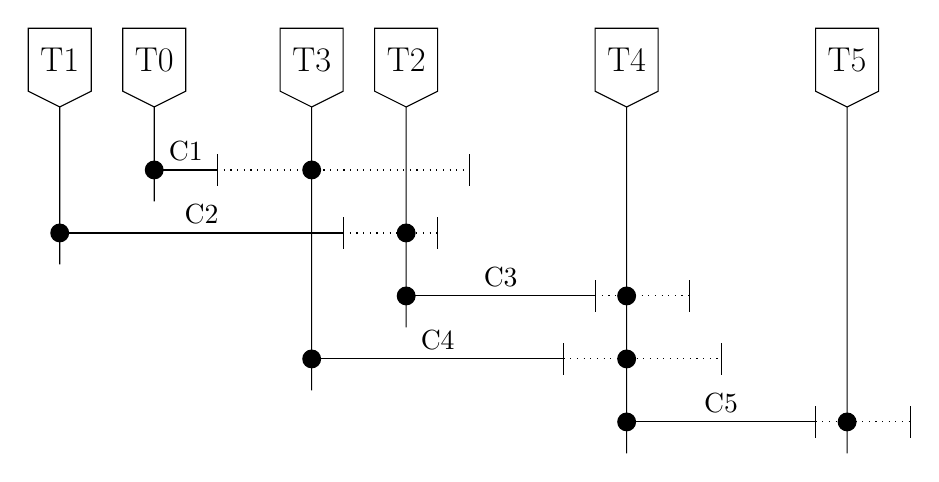
\begin{tikzpicture}[scale=0.4]%
\def\date{0};%
\def\contraintName{C1};%
\def\ypos{-2};%
\def\min{2};%
\def\nom{5};%
\def\max{10};%
\fill (\date,\ypos) circle (0.3);%
\fill (\date+\nom,\ypos) circle (0.3);%
\draw (\date,\ypos) -- ++(\min,0) node[midway,above,scale=1] {\contraintName};%
\draw (\date+\min,\ypos+0.5) -- ++(0,-1);%
\draw[dotted] (\date+\min,\ypos) -- (\date+\max,\ypos);%
\draw (\date+\max,\ypos+0.5) -- ++(0,-1);%
%
\def\nodeName{\Huge T0};%
\def\ypos{-3};%
\draw (\date,0) -- ++(-1,0.5) -- ++(0,2) -- ++(2,0) -- ++(0,-2) -- ++(-1,-0.5) -- (\date, \ypos);%
\draw (\date,1.5) node[scale=0.5]{\nodeName};%
%
\def\date{-3};%
\def\contraintName{C2};%
\def\ypos{-4};%
\def\min{9};%
\def\nom{11};%
\def\max{12};%
\fill (\date,\ypos) circle (0.3);%
\fill (\date+\nom,\ypos) circle (0.3);%
\draw (\date,\ypos) -- ++(\min,0) node[midway,above,scale=1] {\contraintName};%
\draw (\date+\min,\ypos+0.5) -- ++(0,-1);%
\draw[dotted] (\date+\min,\ypos) -- (\date+\max,\ypos);%
\draw (\date+\max,\ypos+0.5) -- ++(0,-1);%
%
\def\nodeName{\Huge T1};%
\def\ypos{-5};%
\draw (\date,0) -- ++(-1,0.5) -- ++(0,2) -- ++(2,0) -- ++(0,-2) -- ++(-1,-0.5) -- (\date, \ypos);%
\draw (\date,1.5) node[scale=0.5]{\nodeName};%
%
\def\date{8};%
\def\contraintName{C3};%
\def\ypos{-6};%
\def\min{6};%
\def\nom{7};%
\def\max{9};%
\fill (\date,\ypos) circle (0.3);%
\fill (\date+\nom,\ypos) circle (0.3);%
\draw (\date,\ypos) -- ++(\min,0) node[midway,above,scale=1] {\contraintName};%
\draw (\date+\min,\ypos+0.5) -- ++(0,-1);%
\draw[dotted] (\date+\min,\ypos) -- (\date+\max,\ypos);%
\draw (\date+\max,\ypos+0.5) -- ++(0,-1);%
%
\def\nodeName{\Huge T2};%
\def\ypos{-7};%
\draw (\date,0) -- ++(-1,0.5) -- ++(0,2) -- ++(2,0) -- ++(0,-2) -- ++(-1,-0.5) -- (\date, \ypos);%
\draw (\date,1.5) node[scale=0.5]{\nodeName};%
%
\def\date{5};%
\def\contraintName{C4};%
\def\ypos{-8};%
\def\min{8};%
\def\nom{10};%
\def\max{13};%
\fill (\date,\ypos) circle (0.3);%
\fill (\date+\nom,\ypos) circle (0.3);%
\draw (\date,\ypos) -- ++(\min,0) node[midway,above,scale=1] {\contraintName};%
\draw (\date+\min,\ypos+0.5) -- ++(0,-1);%
\draw[dotted] (\date+\min,\ypos) -- (\date+\max,\ypos);%
\draw (\date+\max,\ypos+0.5) -- ++(0,-1);%
%
\def\nodeName{\Huge T3};%
\def\ypos{-9};%
\draw (\date,0) -- ++(-1,0.5) -- ++(0,2) -- ++(2,0) -- ++(0,-2) -- ++(-1,-0.5) -- (\date, \ypos);%
\draw (\date,1.5) node[scale=0.5]{\nodeName};%
%
\def\date{15};%
\def\contraintName{C5};%
\def\ypos{-10};%
\def\min{6};%
\def\nom{7};%
\def\max{9};%
\fill (\date,\ypos) circle (0.3);%
\fill (\date+\nom,\ypos) circle (0.3);%
\draw (\date,\ypos) -- ++(\min,0) node[midway,above,scale=1] {\contraintName};%
\draw (\date+\min,\ypos+0.5) -- ++(0,-1);%
\draw[dotted] (\date+\min,\ypos) -- (\date+\max,\ypos);%
\draw (\date+\max,\ypos+0.5) -- ++(0,-1);%
%
\def\nodeName{\Huge T4};%
\def\ypos{-11};%
\draw (\date,0) -- ++(-1,0.5) -- ++(0,2) -- ++(2,0) -- ++(0,-2) -- ++(-1,-0.5) -- (\date, \ypos);%
\draw (\date,1.5) node[scale=0.5]{\nodeName};%
%
\def\date{22};%
\def\nodeName{\Huge T5};%
\def\ypos{-11};%
\draw (\date,0) -- ++(-1,0.5) -- ++(0,2) -- ++(2,0) -- ++(0,-2) -- ++(-1,-0.5) -- (\date, \ypos);%
\draw (\date,1.5) node[scale=0.5]{\nodeName};%
%
\end{tikzpicture}%
}
